\chapter{Physical Experiment}

The simulation software demonstrates that Huang's algorithm and the forward method do a lot to correct for defocus, but does the physical setup yield similar results? Think of the simulation software as tests or a rough draft of a final paper, and the physical demonstration as the final product or copy. The camera in the physical demonstration mimics a human eye with defocus in the real world, and the images captured by the camera are parallel to the images perceived by the retina. We set up the camera as a defocused eye, and will compare performance Huang's algorithm and the forward method for effectiveness in vision-correction.

% Correct this or even switch chapters 5 and 6

\section{Physical Setup}

Here is the physical setup used in our experiment: 

\begin{figure}[ht]
  \centering
  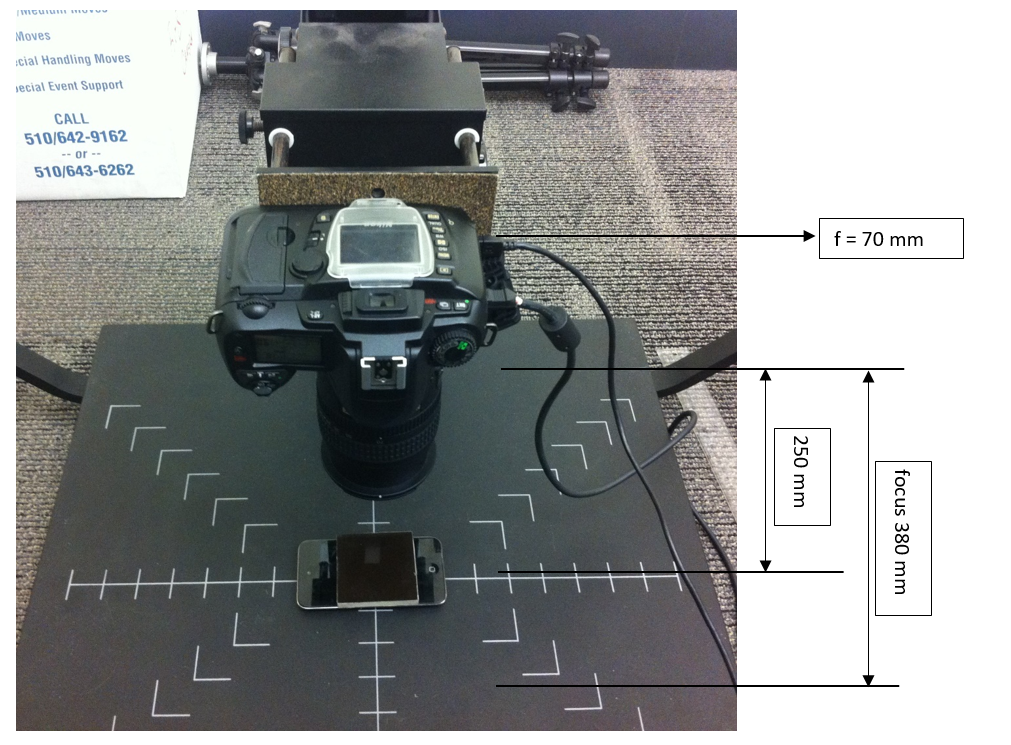
\includegraphics[width=5in]{chapters/chapter5/images/Setup.png}
  \caption{Experimental Setup}
  \label{fig:physical_setup}
\end{figure}
 
We set the f-stop of the camera to f/8, and set the f (zoom) to 70 mm. The distance between the sensor and the flange is 46.5 mm. The camera was focused at 380 millimeters and the distance between the camera and the phone was 250 millimeters. Since the camera focuses farther than the object, our setup simulates mild hyperopia (far-sightedness). This setup closely resembles a +7.69 D defocus, and a +4 D defocus represents a risk factor for adults. 
% http://www.iscreenvision.com/faqs/hyperopia-farsightedness/

% Mention the type of camera I am using

We compare the performance of Huang's algorithm and the forward method. For Huang’s algorithm, the depth of the pinhole mask was 4 millimeters, and for the forward method, the depth was 6 millimeters. Other parameters remained the same for both algorithms. 

\section{Results} 

\begin{table}[!h]
    \caption{Original Images for Reference}
    \begin{tabular}{| l | l }
    \hline Bunny Image & Word Image \\ \hline
      
\includegraphics[width=3in]{chapters/chapter5/images/Clean_Images/0084_820.png} &
      
\includegraphics[width=3in]{chapters/chapter5/images/Clean_Images/Hello.png} \\ \hline
    \end{tabular}
\end{table}


\begin{table}[!h]
    \caption {Huang's Algorithm, Bunny Image}
    \begin{tabular}{| l | l | l |}
    \hline Blurred/Defocused Image & Prefiltered Image & Pinhole-Corrected Image \\ \hline
      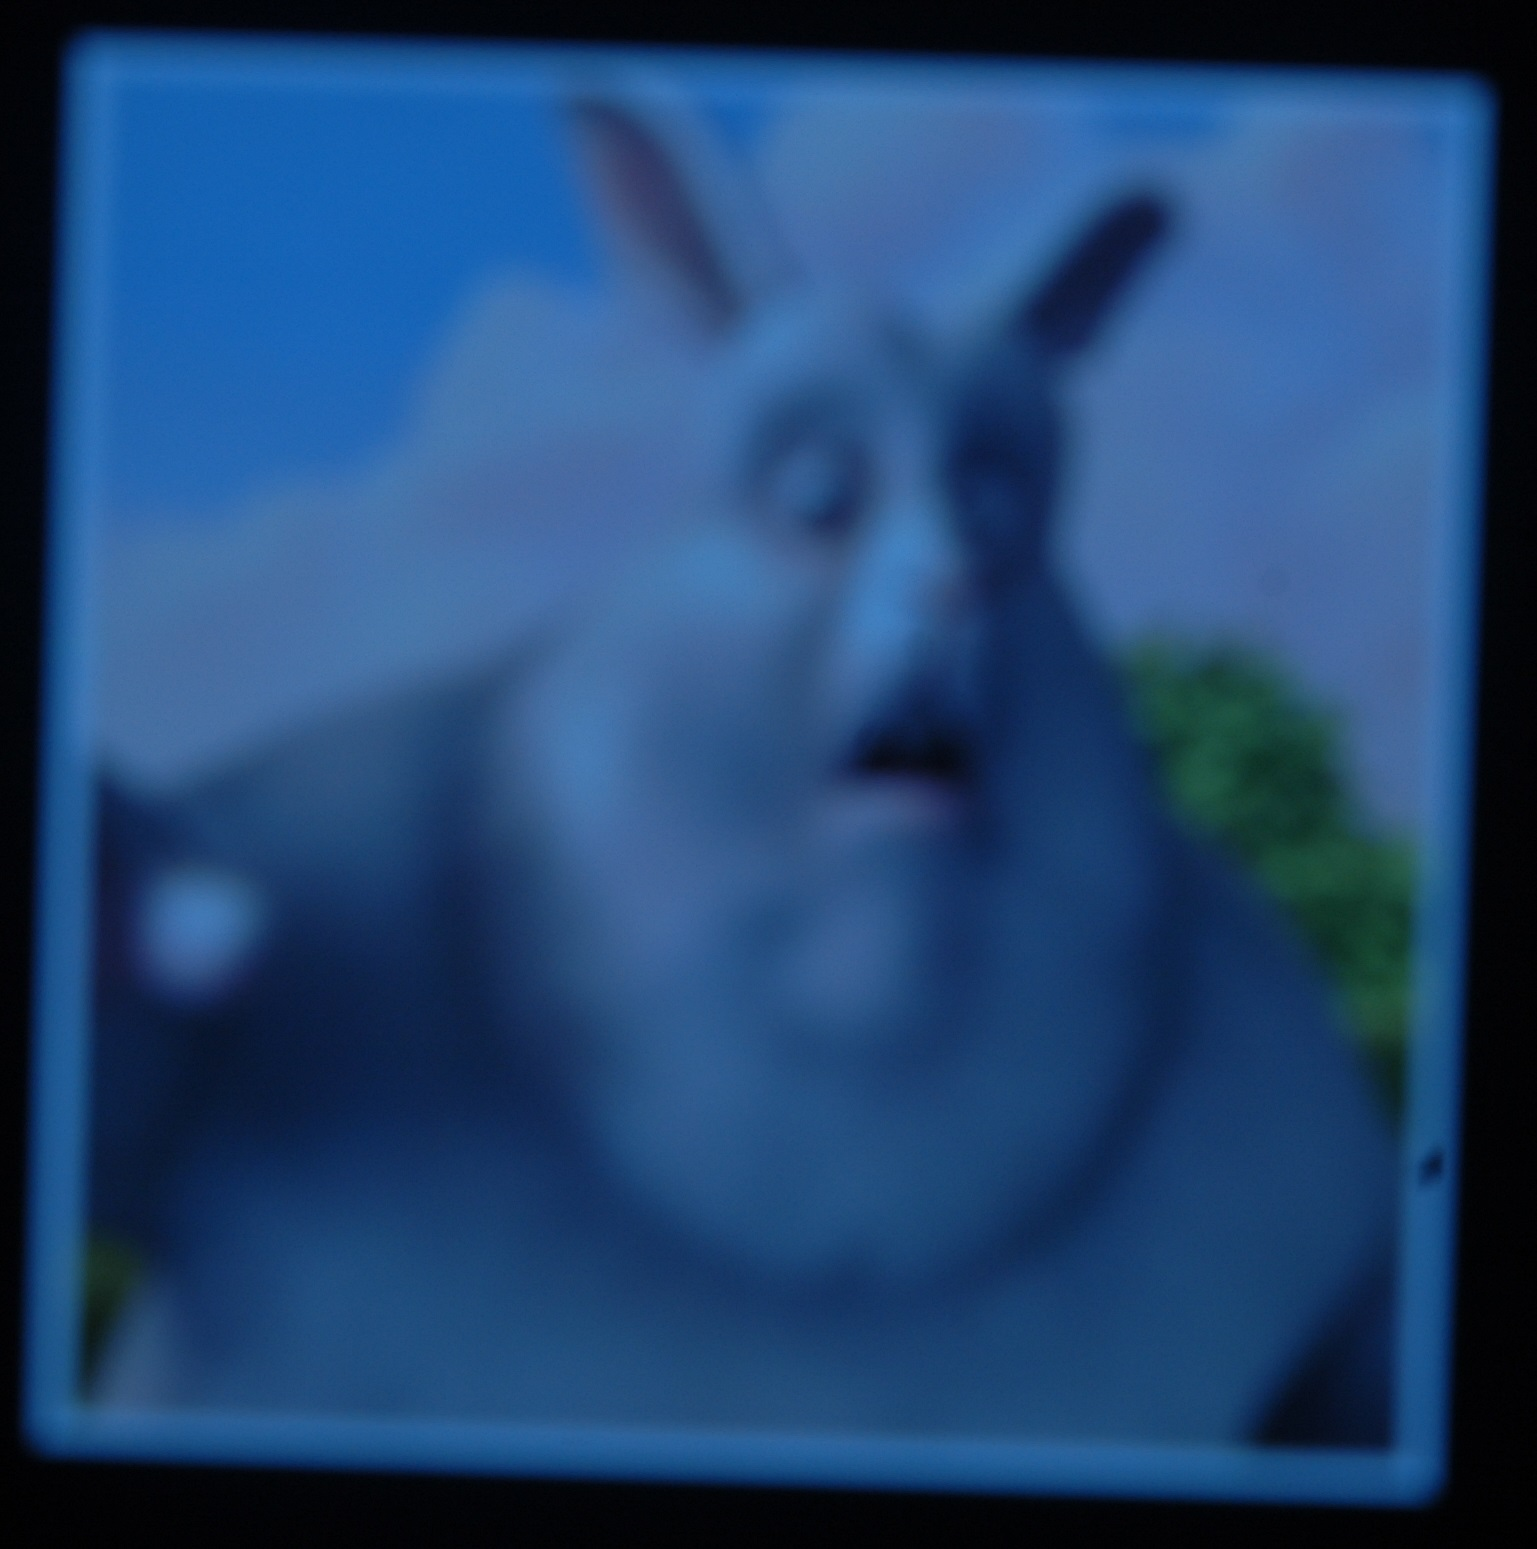
\includegraphics[width=1.9in]{chapters/chapter5/images/Huang_OffAxis_380_250_Origin_Bunny.JPG} &
      \includegraphics[width=1.9in]{chapters/chapter5/images/Huang_prefiltered.PNG} &
      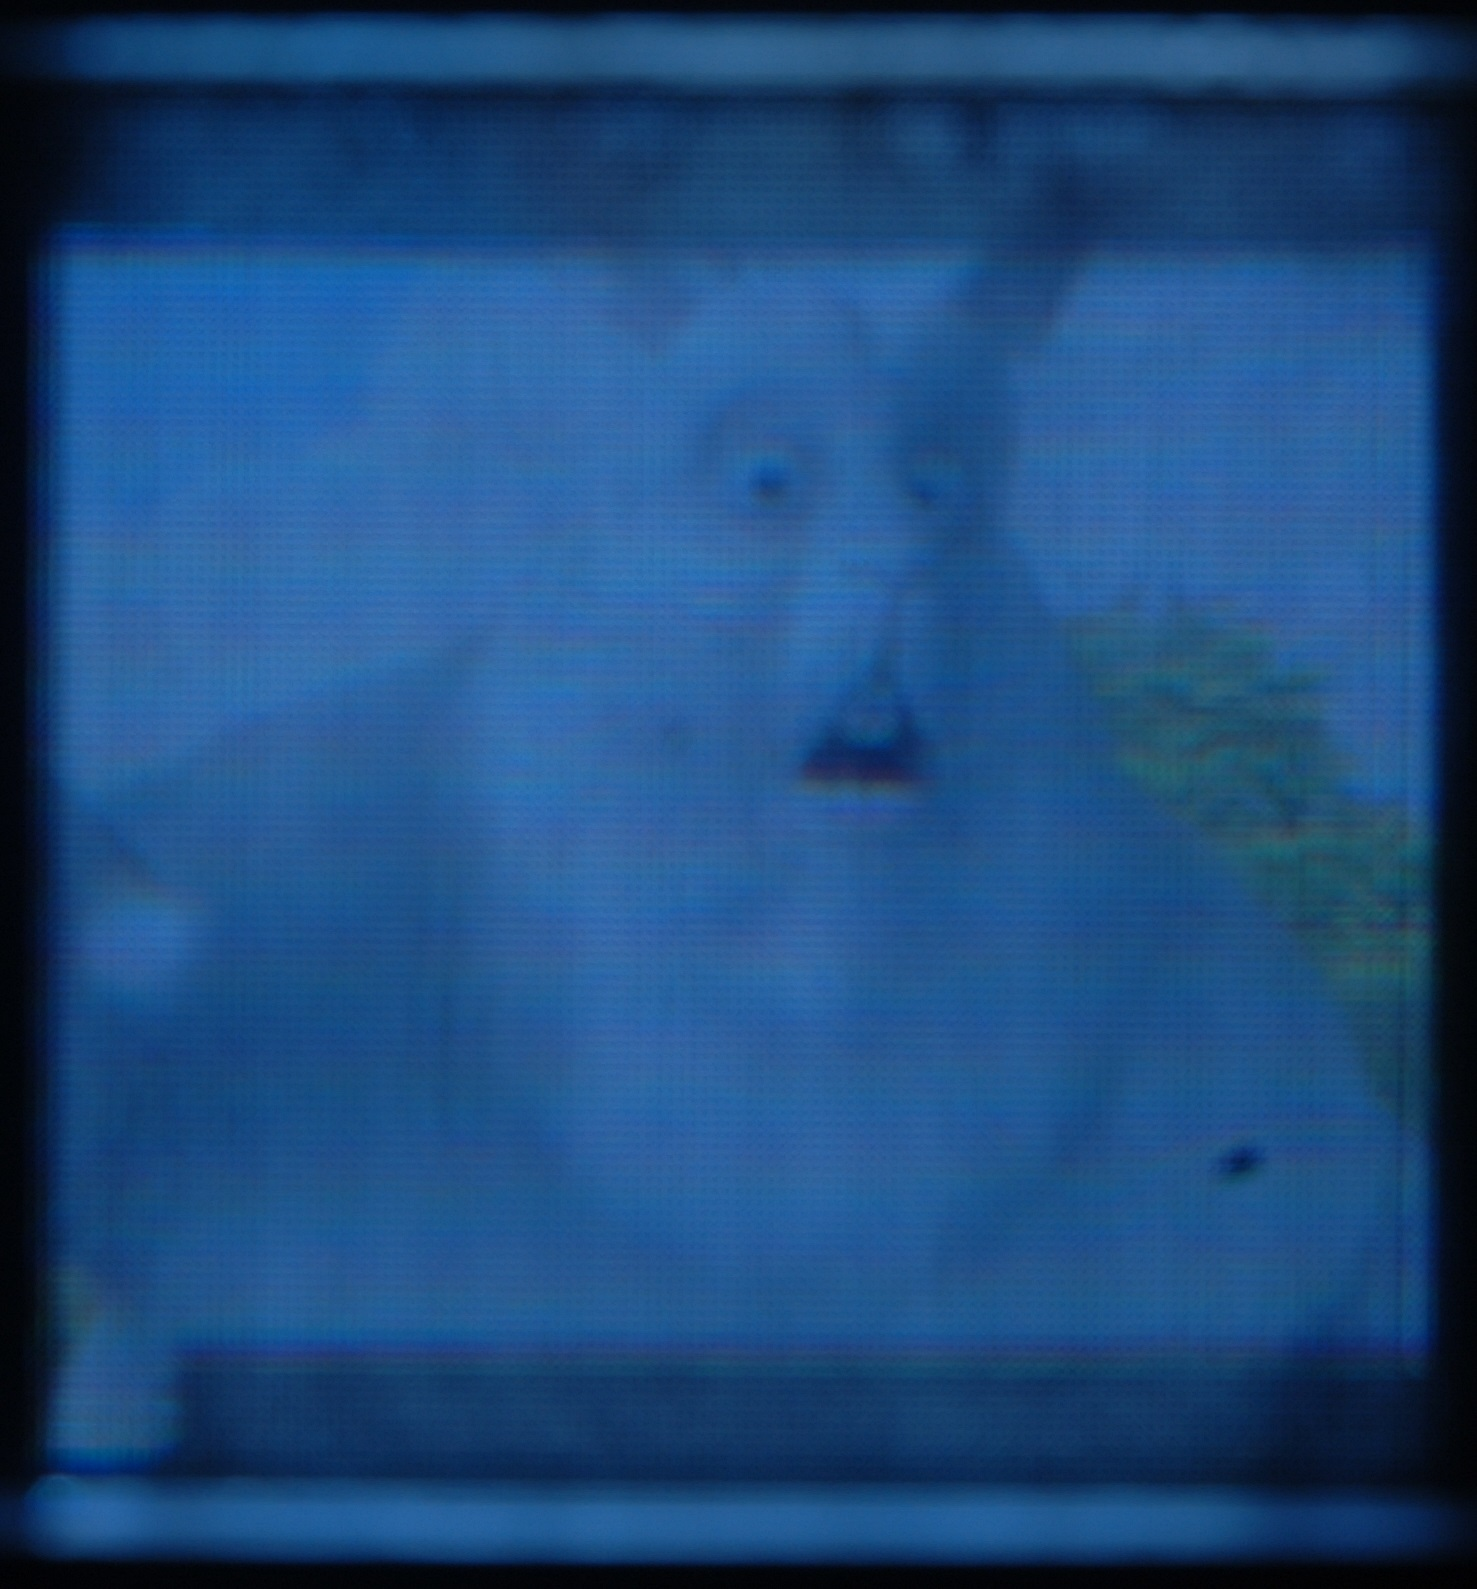
\includegraphics[width=1.9in]{chapters/chapter5/images/Huang_OffAxis_380_250_Pinhole_Bunny.JPG} \\ \hline
    \end{tabular}
\end{table}

\begin{table}
     \caption {Forward Method, Bunny Image}
    \begin{tabular}{| l | l | l |}
    \hline Blurred/Defocused Image & Prefiltered Image & Pinhole-Corrected Image \\ \hline
      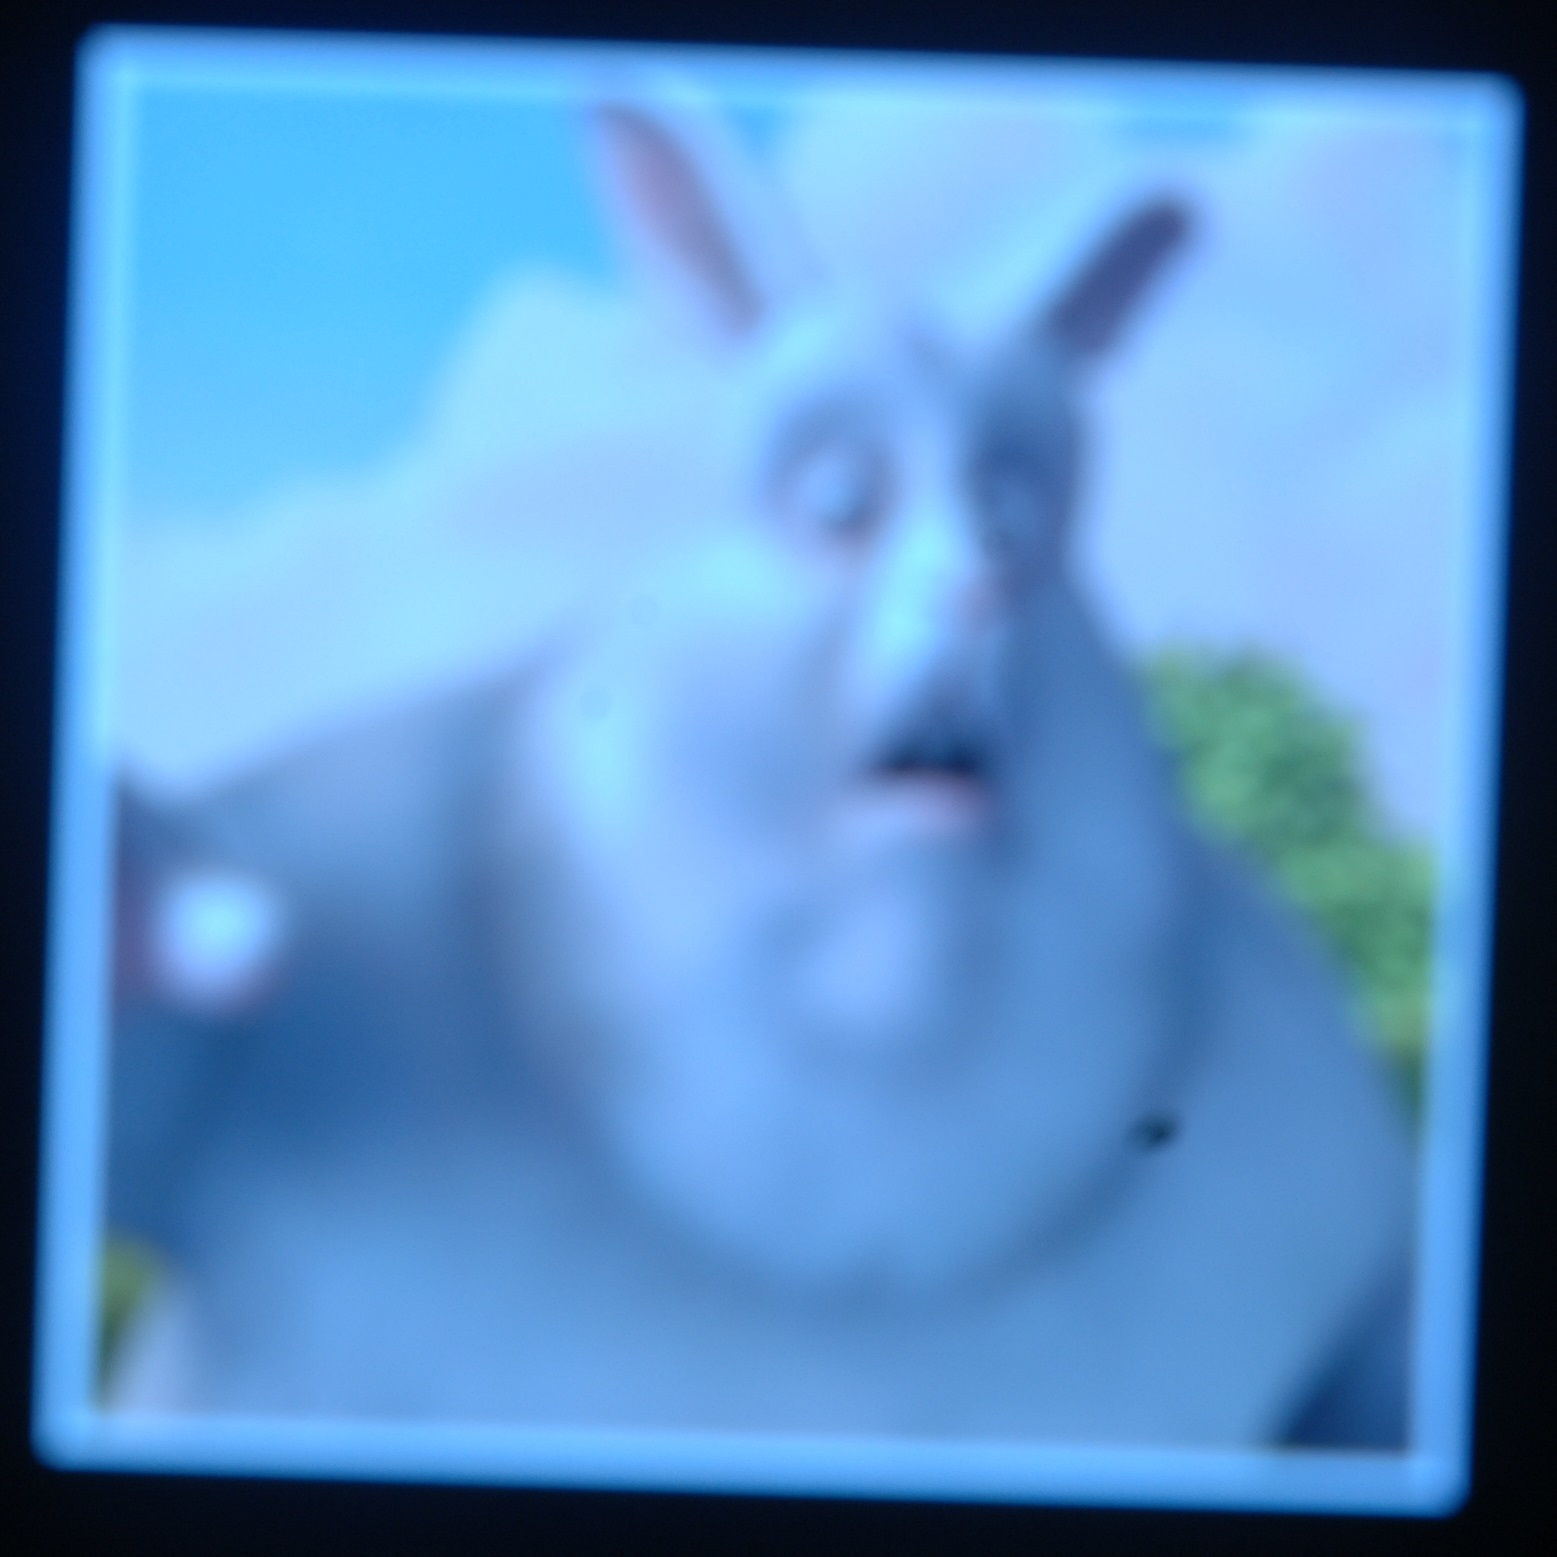
\includegraphics[width=1.9in]{chapters/chapter5/images/Shichao_Bunny_380_250_Origin.JPG} &
      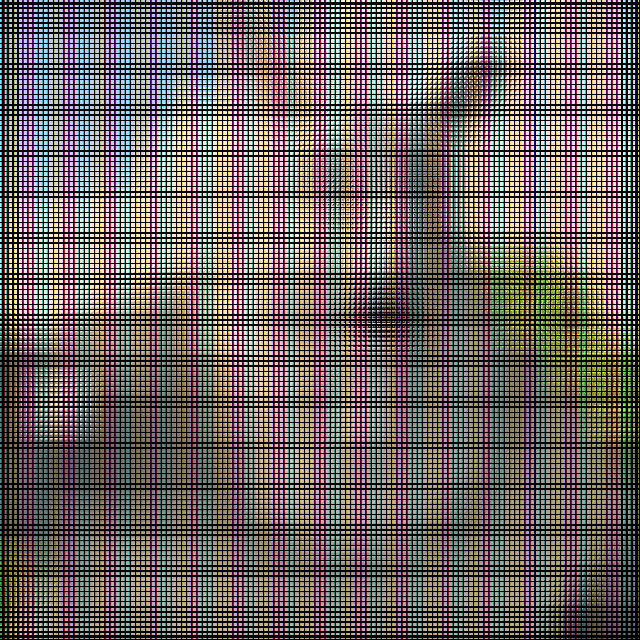
\includegraphics[width=1.9in]{chapters/chapter5/images/Shichao_Bunny_Prefiltered.png} &
      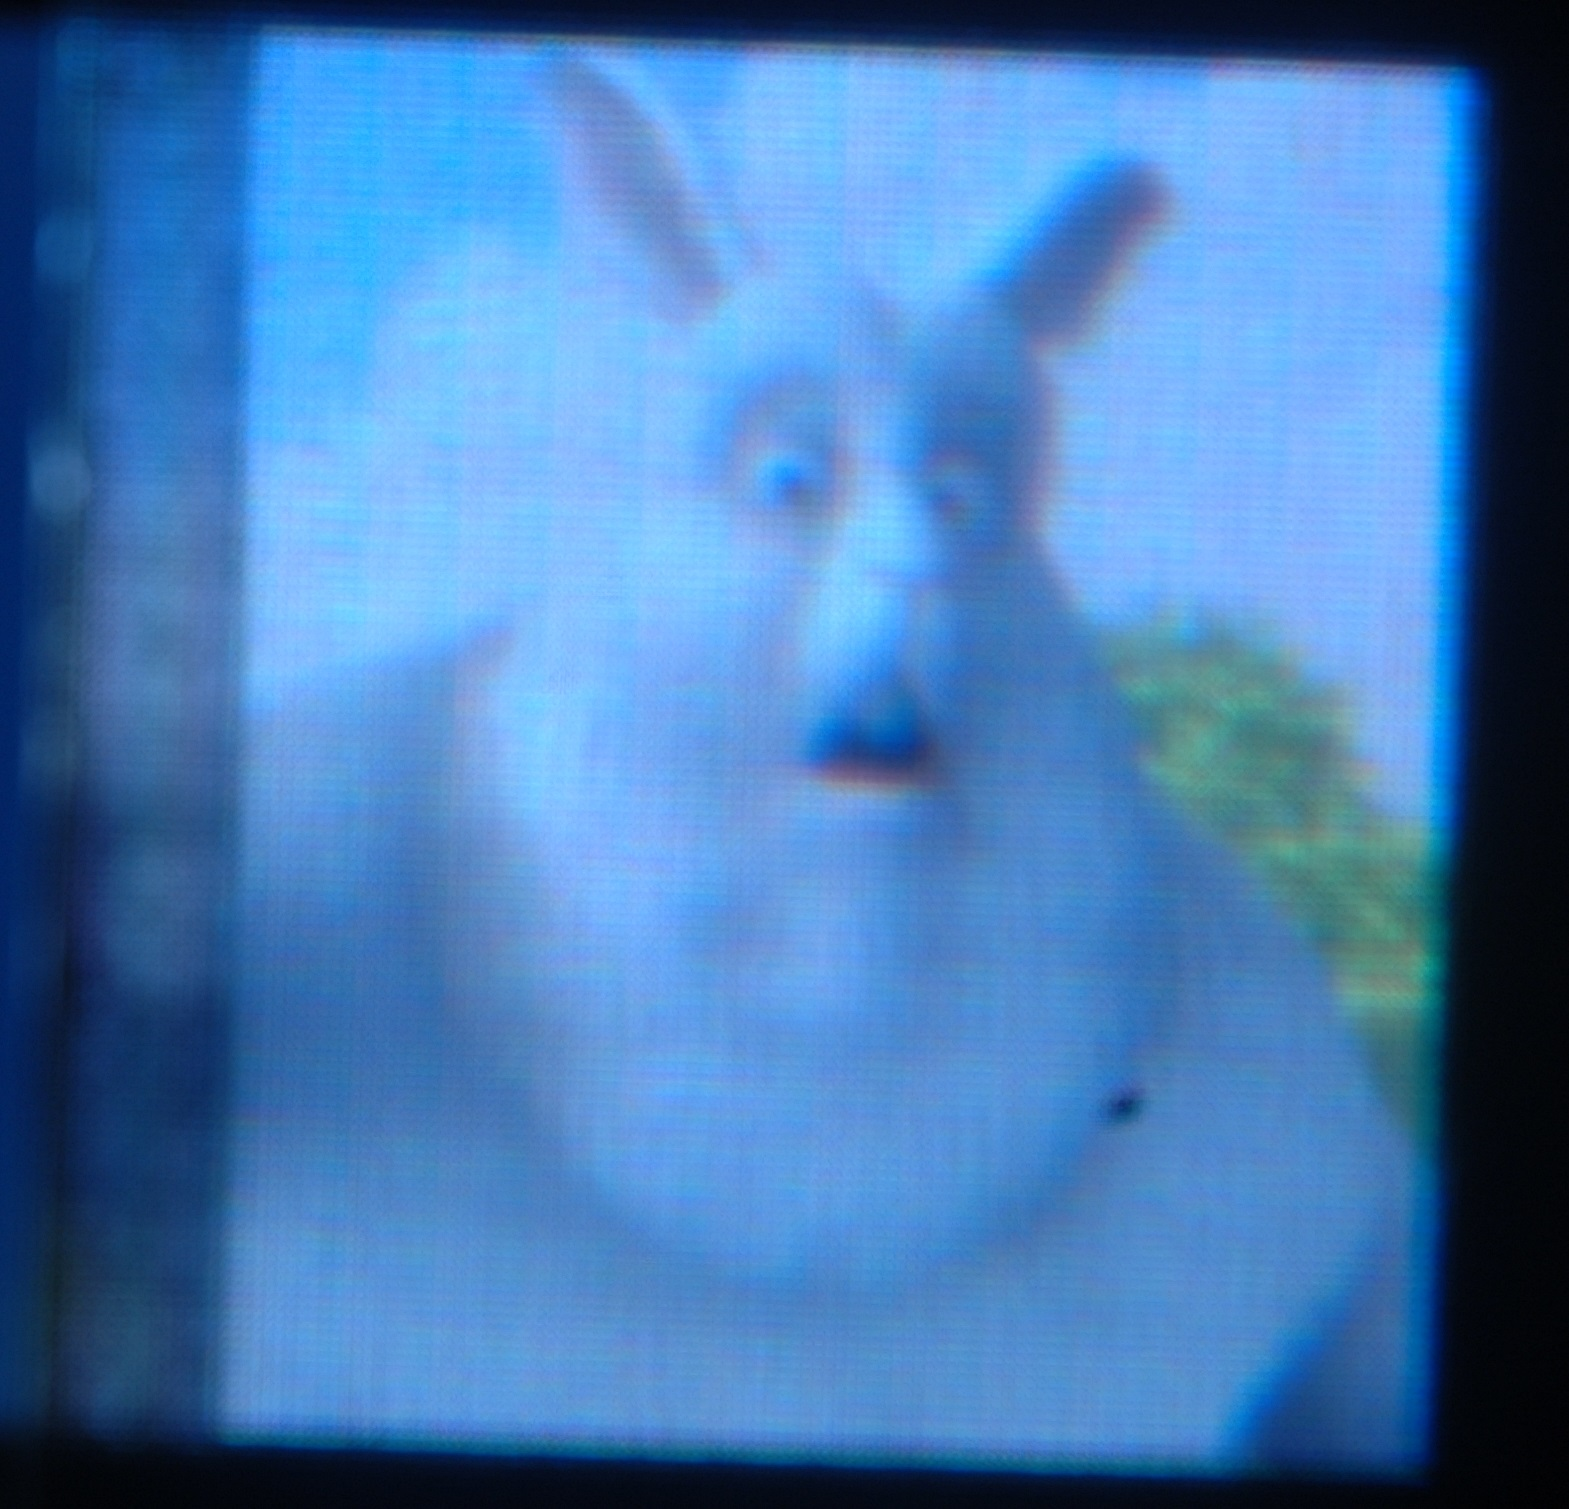
\includegraphics[width=1.9in]{chapters/chapter5/images/Shichao_Bunny_380_250_Pinhole.JPG} \\ \hline
    \end{tabular}
\end{table}
 	 	 
\begin{table}
    \caption {Forward Method, Text Image}
    \begin{tabular}{| l | l | l |}
    \hline Blurred/Defocused Image & Prefiltered Image & Pinhole-Corrected Image \\ \hline
      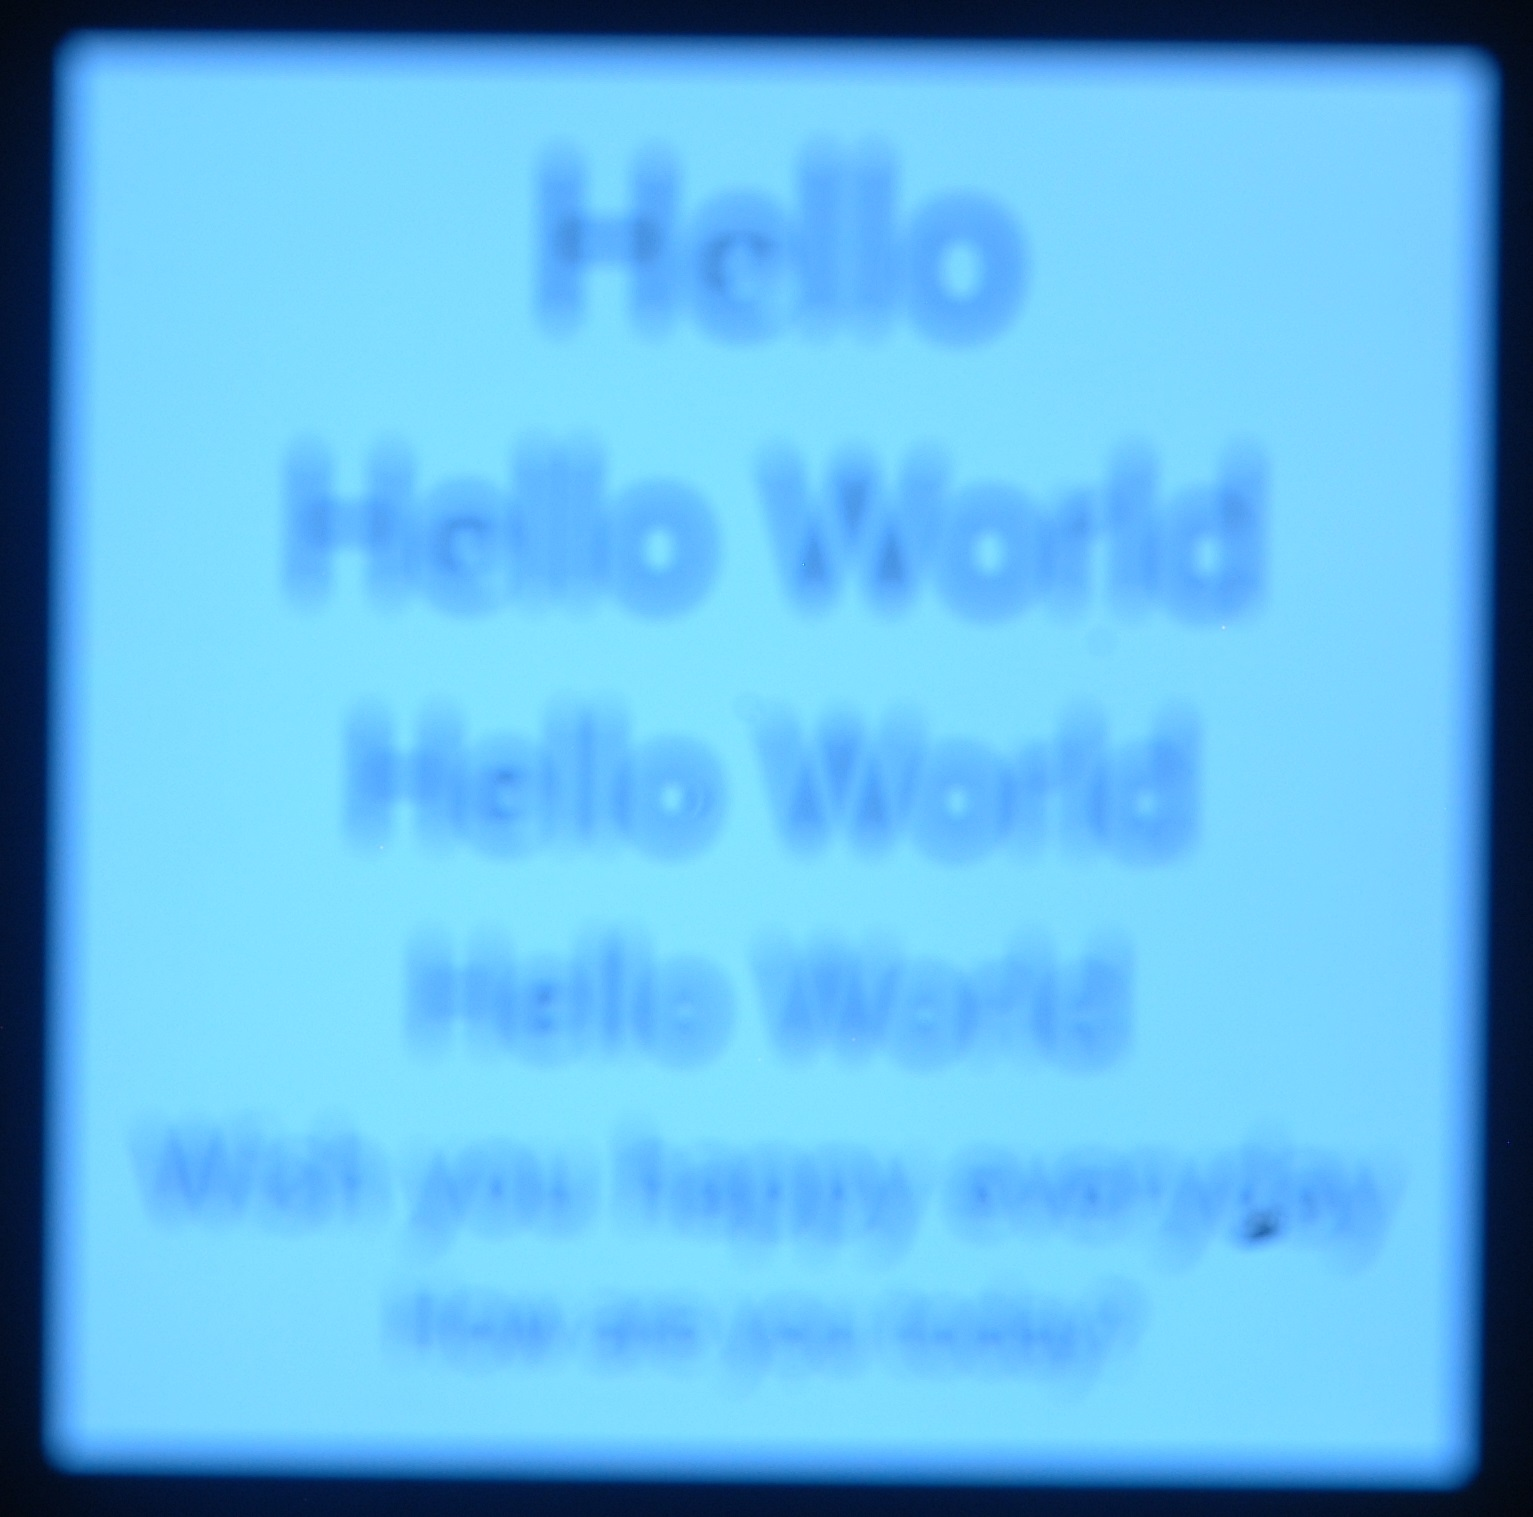
\includegraphics[width=1.9in]{chapters/chapter5/images/Shichao_Words_380_250_Origin.JPG} &
      \includegraphics[width=1.9in]{chapters/chapter5/images/Shichao_word_Prefiltered.png} &
      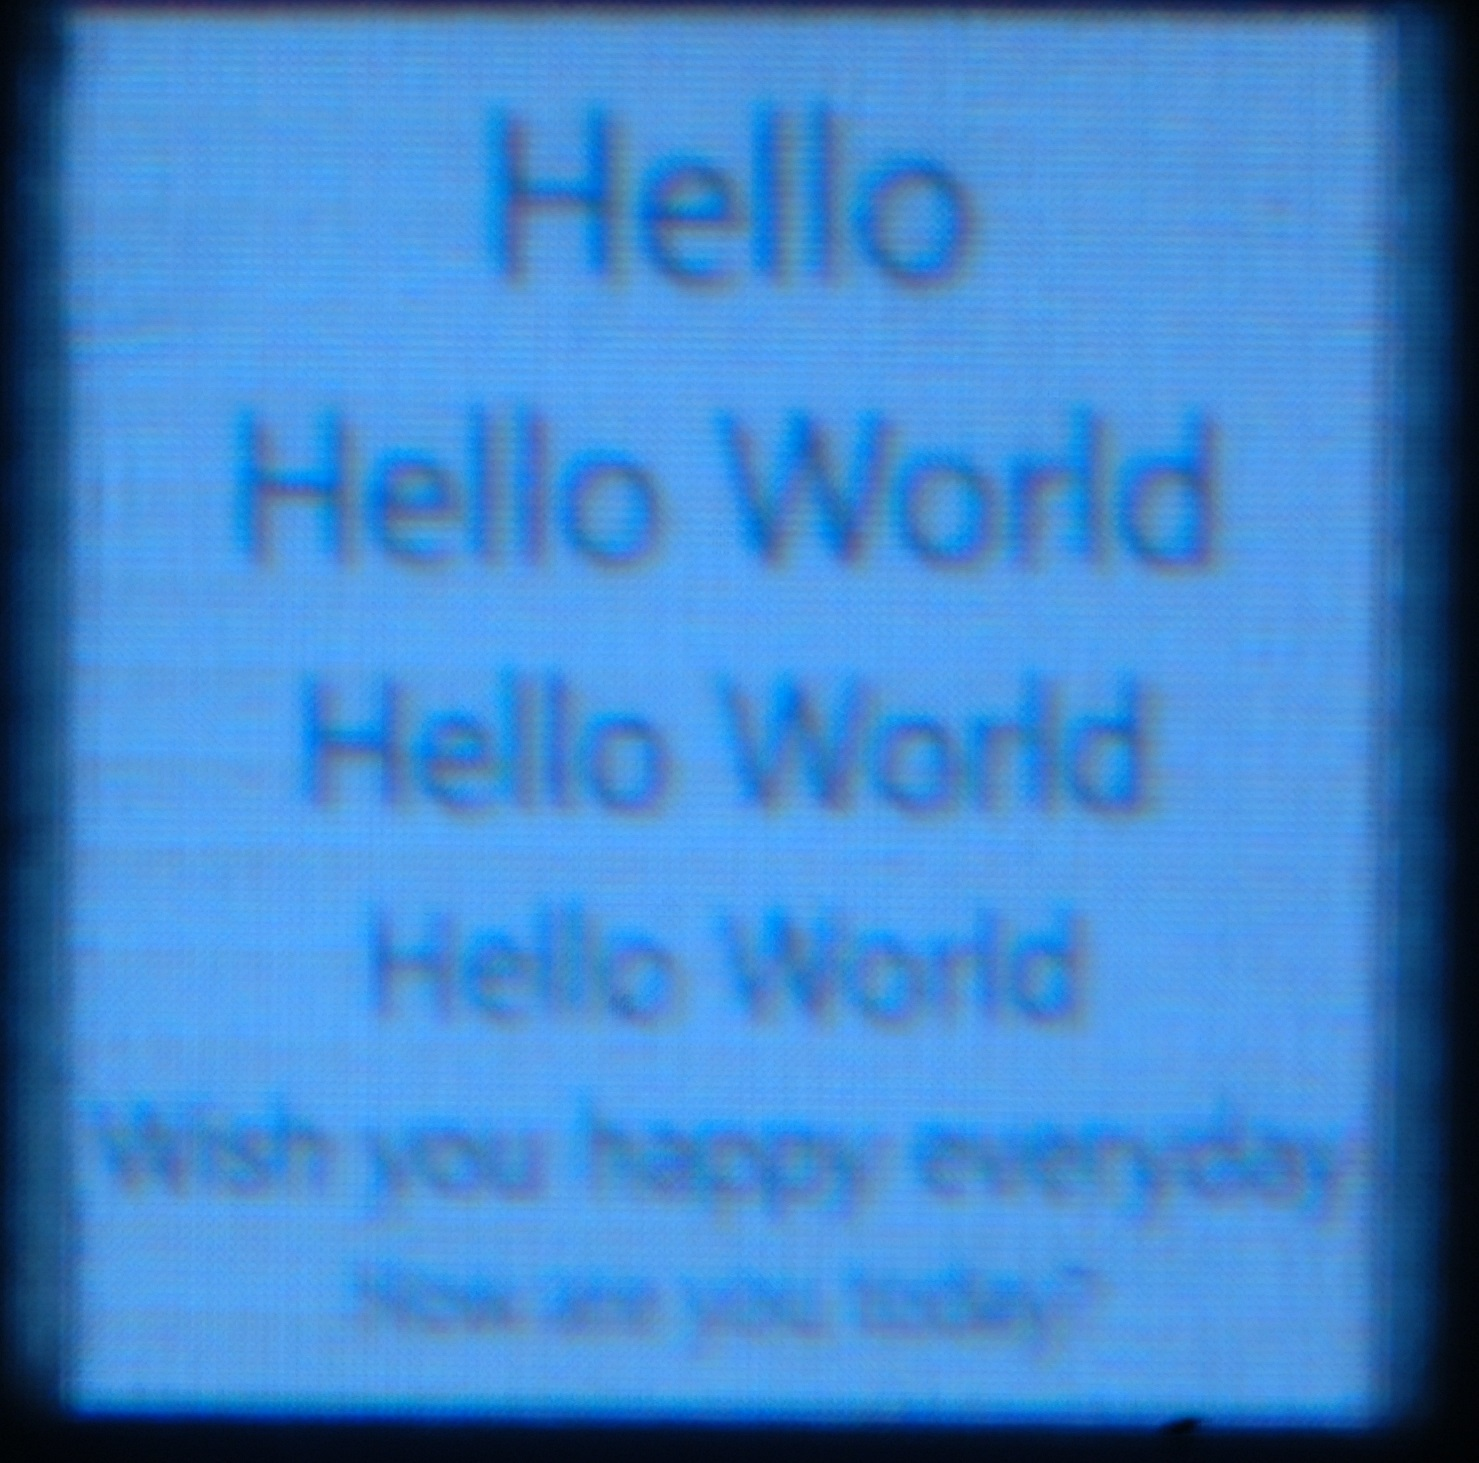
\includegraphics[width=1.9in]{chapters/chapter5/images/Shichao_Words_380_250_Pinhole.JPG} \\ \hline
    \end{tabular}
\end{table} 

\newpage
\section{Analysis}

For Huang’s algorithm, the corrected image shows better resolution but worse contrast. The bunny is far more clear in the corrected image than the defocused image, but the sky becomes saturated. Nevertheless, an average user would likely prefer the corrected image. 

For the forward method, the bunny image shows moderately better resolution with little to no change in contrast. The forward method yields slightly less improvement in resolution than Huang’s algorithm, but the limited loss of contrast makes the forward method more appealing depending on the viewer.

The forward method performs best on the text image in terms of resolution and contrast. In the defocused image, the last three lines are nearly impossible to read, and all words are badly blurred. However, in the corrected image, the first 3 lines are very clear, the next two lines are readable, and only the final line is blurry. 

We adjusted the image brightness on the cell phone and the exposure time of the camera that yielded the best possible results, so we did not keep the brightness factor constant. Nevertheless, exposure time was kept between 1.5 seconds and 2 seconds, so the differences in brightness between images was not significant. In the real world, a user has the ability to adjust the brightness on their cell phone, and a human eye is capable of adjusting to different light conditions. 

\section{Conclusion and Future Work}
For this specific case – an object placed 250 millimeters away and focused at 380 mm – both Huang’s algorithm and the forward method yield improvements in quality of image. In the bunny image, Huang’s algorithm yields slightly better resolution than the forward method but at the cost of losing contrast. The improvement in text image in the forward method is especially appealing because users usually spend more time reading text on an iPhone than viewing images. 
In the future, we want to run experiments on other object distances, focus distances, and depths. For example, we may want to try to simulate myopia (nearsightedness) – focus at 380 mm but place the object 500 mm away. Moreover, we want to do physical experiments with higher-order aberrations, which is much more challenging.